\chapter{Design}

\section{Portable Document Format}
In the context of text redaction, it is essential to consider the relevant components that make up a PDF document and influence security for direct redaction in the document. We consider the PDF document type which contains text data for both the font and the layout of each character (glyph) on a page. 

\subsection{Structure}
A PDF document can be split into 4 distinct parts: 
\\\\
\textbf{Header}. The header of a PDF document serves as its starting point. It contains the critical information about the file which is essential for identifying the PDF format and ensuring compatibility with PDF readers. \\
\textbf{Trailer}. The trailer is found at the end of the document and provides essential information for reading and processing the document. It includes the number of entries in the cross-reference table. It references to the root object of the document's catalog, which contains information about the document's structure, outlines and elements. Finally it may include additional information about encryption, digital signatures and metadta if present. \\
\textbf{Cross-Reference Table(Xref)}. The Cross-Reference Table maintains a record of the location and structure of all objects within the PDF. The Xref table enables efficient random access and editing of the document. It lists the objects, their byte offsets within the file and information about whether an object is in use of has been deleted. \\
\textbf{Body}. The body is where the actual content resides. It includes everything that is visible within the document. This includes text, images, graphical elements, forms and more. The content of a PDF is organized into objects. 
\\\\
The actual contents of a page are often embedded through a stream. A stream may be contained in an object and consists of a sequence of operators with operands which may refer to other objects or information elsewhere.
\begin{figure}[h]
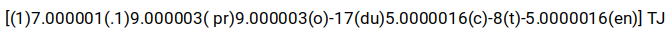
\includegraphics[width=0.85\textwidth]{latex/media/TJexample.png}
\centering
\caption{The TJ text showing operator specifies the glyphs to render, along with their widths and associated positional adjustments by the reference to a font object (not shown here). Adjustments are given in text space units. }
\label{fig:tjexample}
\end{figure}
\subsection{Text rendering}
PDF documents can render text in a wide range of ways, including by the use of a text showing operator such as TJ or Tj. The TJ operator takes as arguments a string of text and a vector of positional adjustments which displace the character with respect to its default position. This position is often determined by the previous character on the line, consisting of a fixed offset that is equivalent to the \textit{advance width} of the previous character. Figure \ref{fig:tjexample} is an example of a TJ text showing operator in practice.
\\\\
Glyph advance widths and glyph shifts create a security concern. The exact width of a redaction and any non-redacted glyph shifts conditioned on redacted glyphs may be used to eliminate potential redacted texts. \cite{bland2022story}. Documents may or may not have these positional adjustments based on the \textit{workflow} that has been used. When saving an email or using 'Save as PDF' in Microsoft Word for example, the documents have \textit{dependent} shifting schemes, while other workflows may produce documents which are \textit{unadjusted}.

\subsubsection{Redaction width}


\subsection{Metadata}
A PDF document may contain extra 'hidden' information which is contained within the metadata of the document. This metadata may contain information about the actual textual contents of the document (figure \ref{fig:metadataexmp}). An example are annotations by authors or reviewers which may comment on a specific part of the document, referring or quoting text which has been redacted from the page, but not from the document. 
\begin{figure}[h]
    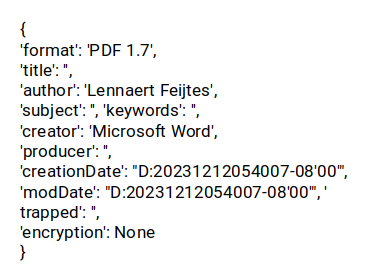
\includegraphics[width=0.5\linewidth]{latex/media/metadata.png}
    \centering
    \caption{An example of metadata which may be present in a PDF document. Information such as the author name, subject and description of the document can be retrieved if not also removed.}
    \label{fig:metadataexmp}
\end{figure}\\
The table of contents, embedded files, XML metadata and internal links are also hidden to the eye but may contain sensitive information even after redaction. This information may include author names, document descriptions, links or other references to sensitive personal information which has not been correctly removed.

\section{A new redaction method?}
The process of safely redacting information from a document consists of multiple steps. To redact text, it has to be removed from the PDF by manipulating the content stream of a page.
Parts of a content stream have to be removed or updated, including both string values and positional information about the text. Furthermore, the positional information of the other words on the line have to be adjusted to reduce the leaked information. This is a difficult task because words may be broken up in different text rendering operations, text may be split up in multiple content streams and determining the actual position of a to-be-redacted word can be complicated depending on the workflow used. 
\\\\
For small words